\documentclass{article}

\usepackage{upgreek}

\usepackage{parskip}

\sloppy

\usepackage{amsmath} % actually amsopn
\makeatletter
\DeclareRobustCommand{\var}[1]{\begingroup\newmcodes@\mathit{#1}\endgroup}
\makeatother
\makeatletter
\DeclareRobustCommand{\varb}[1]{\begingroup\newmcodes@\mathbf{#1}\endgroup}
\makeatother

\usepackage{amsfonts}

\usepackage[a4paper, margin=1in]{geometry}

\usepackage{mathtools}
\DeclarePairedDelimiter\ceil{\lceil}{\rceil}
\DeclarePairedDelimiter\floor{\lfloor}{\rfloor}
\DeclarePairedDelimiter\chevrons{\langle}{\rangle}

\usepackage{graphicx}
\graphicspath{{./}}

\usepackage{color}

\definecolor{hyperref}{rgb}{0, 0, 0.4}
\usepackage{hyperref}
\hypersetup{
	colorlinks=true,
	urlcolor=hyperref,
	}

\usepackage[section]{placeins}

\newcommand{\n}{\ \-}

\usepackage{enumitem}

\usepackage[style=ieee]{biblatex}
\addbibresource{refs.bib}

\usepackage{algorithm}
\usepackage{algpseudocode}

\MakeRobust{\Call}

\begin{document}

\section*{Introduction}

This report outlines and analyses an implementation of a parallel algorithm for the following
problem:\\
Given a grid, where each square has a positive integer as its cost, find the shortest 8 connected
path from the top left most square to the bottom right most square, where the distance of a path is
defined as the sum of costs of all squares on the path.

The algorithm I've devised is a modified version of the delta stepping algorithm from Mayer and
Sanders \cite{Meyer-1998}, described in the algorithm 1 with its functions in algorithm 2.
\begin{algorithm}
	\caption{}
	\begin{algorithmic}[1]
		\State \(x_{end}\gets x_{size} - 1\)
		\State \(y_{end}\gets y_{size} - 1\)

		\State \(delta\gets \Call{FindDelta}{ }\)
		\For{\(x \gets 0\) \textbf{to} \(x_{end}\)}\textbf{ in parallel}
			\For{\(y \gets 0\) \textbf{to} \(y_{end}\)}\textbf{ in parallel}
				\State $distance[x][y] \gets \infty$
				\State $bmap[x][y] \gets -1$ \Comment{bmap map (x, y) to the which b[i] set they're
				in, hence speeding up the \textsc{Remove}.}
			\EndFor
		\EndFor

		\State \(distance[0][0]\gets \Call{Cost}{0, 0}\)
		\State \Call{Insert}{0, 0}

		\State $i_{dest} \gets \infty$
		\State $removed \gets \emptyset$
		\State $relaxed \gets \emptyset$

		\State $i \gets 0$
		\While{$i < i_{dest}$}
			\While{b[i] is not empty}
				\State \Call{Relax}{b[i], relaxed, removed}
				\State $b[i] \gets \emptyset$
				\For{$\textbf{each} (x, y) \in relaxed$} \textbf{in parallel}
					\State \Call{Insert}{x, y}
					\If{$ x_{end} = x \land y_{end} = y $}
						\State $i_{dest} \gets i$
					\EndIf
				\EndFor
			\EndWhile
			\State $relaxed \gets \emptyset$
			\State $removed \gets \emptyset$
		\EndWhile

		\State $x \gets x_{end}$ \Comment{Reconstruct the path from distance.}
		\State $y \gets y_{end}$
		\State $path \gets [ ]$
		\While{$x \ne 0 \land y \ne 0$}
			\State $x_{pred} \gets x$
			\State $y_{pred} \gets y$
			\For{\(dx \gets -1, 0, 1\)}
				\For{\(dy \gets -1, 0, 1\)}
			\State $x_{new} \gets x + dx$
			\State $y_{new} \gets y + dy$
					\If{\((x_{new}, y_{new}) \text{ is valid coordinate} \land (x_{new},
					y_{new}) \ne (x, y)\)}
						\If{$distance[x_{new}][y_{new}] < distance[x_{pred}][y_{pred}]$}
							\State $x_{pred} \gets x_{new}$
							\State $y_{pred} \gets y_{new}$
						\EndIf
					\EndIf
				\EndFor
			\EndFor
			\State $path prepend (x_{pred}, y_{pred})$
		\EndWhile
		\State \Return path
	\end{algorithmic}
\end{algorithm}
\begin{algorithm}
	\caption{Functions of Algorithm 1}
	\begin{algorithmic}[1]
		\Function{FindDelta}{ }
			\For{\(x \gets 0\) \textbf{to} \(x_{end}\)}\textbf{ in parallel}
				\For{\(y \gets 0\) \textbf{to} \(y_{end}\)}\textbf{ in parallel}
					\State \(cost_{max} \gets \Call{Max}{cost_{max}, \Call{Cost}{x, y}}\)
				\EndFor
			\EndFor
			\State \Return \(cost_{max} / 8\)
		\EndFunction
		\Function{Remove}{x, y}
			\If{$bmap[x][y] \ne -1$}
				\State $b[bmap[x][y]] \gets b[bmap[x][y]] \setminus {(x, y)}$
			\EndIf
		\EndFunction
		\Function{Insert}{x, y}
			\State $i \gets \floor{distance[x][y] / delta}$
			\State $bmap[x][y] \gets i$
			\State $b[i] \gets b[i] \cup (x, y)$
		\EndFunction

		\Function{Relax}{to-relax, relaxed, removed} \Comment{pass NULL as removed will cause the
		function to only Relax heavy edges. Pass a set as removed will cause the function to call
		\textsc{Remove} for each coordinate in to-relax and add them to removed.}
			\For{\textbf{each} \((x, y) \in \) to-relax} \textbf{in parallel}
				\If{\(removed \ne NULL\)}
					\State \Call{Remove}{x, y}
					\State \(removed \gets removed \cap (x, y)\)
				\EndIf
				\For{\(dx \gets -1, 0, 1\)}
					\For{\(dy \gets -1, 0, 1\)}
						\State \(x_{next} \gets x + dx\)
						\State \(y_{next} \gets y + dy\)
						\If{\((x_{next}, y_{next}) \text{ is valid coordinate} \land (x_{next},
						y_{next}) \ne (x, y)\)}
							\If{$(\Call{Cost}{x_{next}, y_{next}} \le delta) \oplus (removed =
							NULL)$} \Comment{If removed is null, only relax heavy edges, otherwise
							only relax light edges.}
								\State $distance_{new} \gets distance[x][y] + \Call{Cost}{x_{next},
								y_{next}}$
								\If{$distance_{new} < distance[x_{next}][y_{next}]$}
									\State $distance[x_{next}][y_{next}] \gets distance_{new}$
									\State $relaxed \gets relaxed \cap (x_{next}, y_{next})$
								\EndIf
							\EndIf
						\EndIf
					\EndFor
				\EndFor
			\EndFor
		\EndFunction
	\end{algorithmic}
\end{algorithm}

Note that \(\Call{Cost}{x, y}\) returns the cost of the cell on \(x_{th}\) row and \(y_{th}\).
Furthermore, while the cost takes a long time to calculate for the first time. This function caches
the cost in a 2D array so subsequence call returns instantly. This has the additional effect of
calculating the cost of each cell upfront in a parallel fashion during the \textsc{FindDelta}
procedure. Not only does this allow delta to be calculated at the optimal value. It also allows the
load of calculating the cost of each cell to be spread evenly among all processors, taking advantage
of parallelization for the most expensive part of the algorithm.

Furthermore, to ensure that $relaxed$ and $removed$ can be queried in constant time as well as being
made emptied in constant time, I implemented them as 2D int arrays where (x, y) is in the set if
$set[x][y] = trueValue$. Here $trueValue$ is an integer. By incrementing $trueValue$ we can empty
the set very quickly.

The implementation of the algorithm is less than ideal. Because I choose to use vector in the C++
standard library, which isn't thread safe, I have to heavily used locking and OpenMP critical
region to ensure data races does not happen. This means the implementation of the algorithm isn't as
parallel as it should be and further improvement on data structures and hence performance can be
made.

\section*{Methodology}
To confirm and measure the performance of my algorithm, I've run the algorithm's implementation on
spartan with 1, 2, 4, 8, 16, 32 and 72 threads respectively. The input samples I used are 10x10edge,
10x10expensive, 10x10fast, 10x10faster, 10x10zigzag, 4x4edge and 4x4Z. Among those input samples,
10x10expensive, 10x10fast and 10x10faster are three relatively similar samples with their only
significant difference between each other being the cost of calculating the cost of a cell. These
three samples will provide us with insight over how the overall runtime changes with different cost
of calculating the cost of cells. I've also run a sequential Dijkstra's algorithm implementation
with the same hardware to act as baseline to further evaluate the performance of my delta stepping
algorithm.

I have collected the following metrics of performance:
\begin{itemize}
	\item The overall time taken to run the algorithm.
	\item The overall time taken to calculate the delta, which should be approximately the overall
		time taken to calculate all costs of cells.
	\item The amount of CPU time used to run the whole algorithm. This should be a good
		approximation of the amount of work done by the algorithm.
	\item The amount of CPU time used to calculate all costs of cells. This should be a good
		approximation of the amount of work done to calculate the costs of cells.
\end{itemize}

\section*{Experiments}
\begin{figure}[!htb]
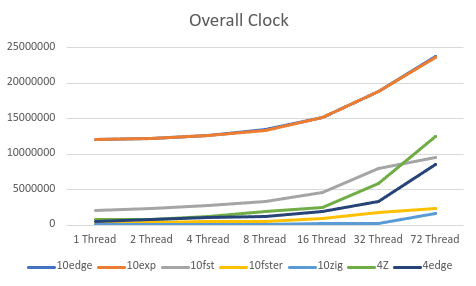
\includegraphics[width=\textwidth]{overall-clock.png}
\caption{Clock Ticked Overall}
\label{fig:1}
\end{figure}

\begin{table}[!htb]
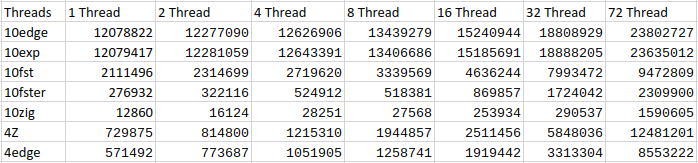
\includegraphics[width=\textwidth]{overall-clock-table.png}
\caption{Clock Ticked Overall}
\label{tab:1}
\end{table}

\begin{figure}[!htb]
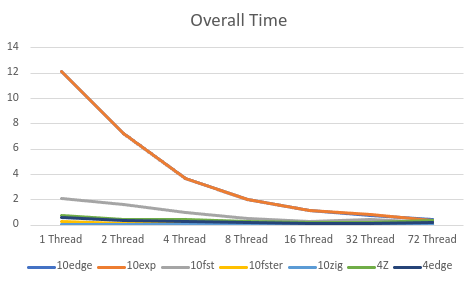
\includegraphics[width=\textwidth]{overall-time.png}
\caption{Time Taken Overall}
\label{fig:2}
\end{figure}

\begin{table}[!htb]
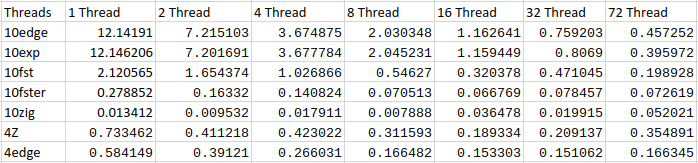
\includegraphics[width=\textwidth]{overall-time-table.png}
\caption{Time Taken Overall}
\label{tab:2}
\end{table}

\begin{figure}[!htb]
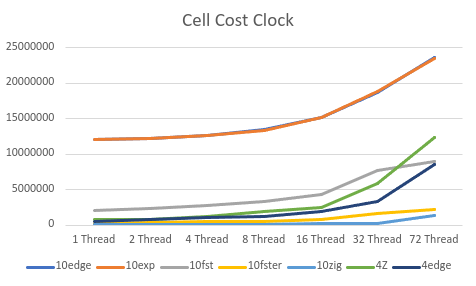
\includegraphics[width=\textwidth]{cell-cost-clock.png}
\caption{Clock Ticked Calculating Cell Cost}
\label{fig:3}
\end{figure}

\begin{table}[!htb]
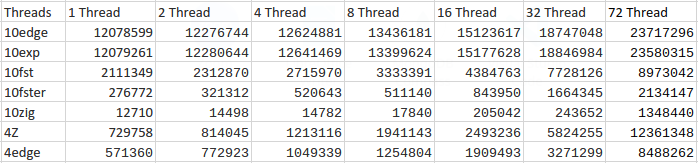
\includegraphics[width=\textwidth]{cell-cost-clock-table.png}
\caption{Clock Ticked Calculating Cell Cost}
\label{tab:3}
\end{table}

\begin{figure}[!htb]
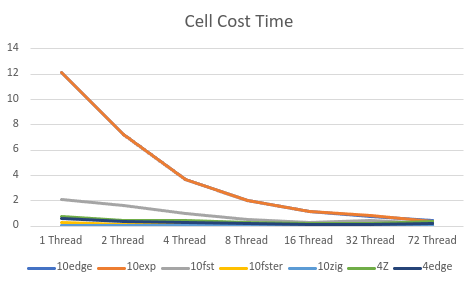
\includegraphics[width=\textwidth]{cell-cost-time.png}
\caption{Time Taken Calculating Cell Cost}
\label{fig:4}
\end{figure}

\begin{table}[!htb]
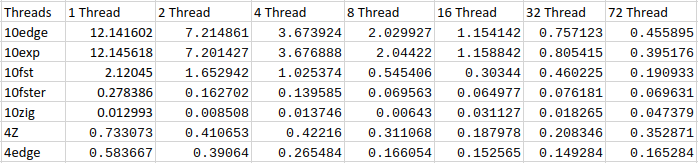
\includegraphics[width=\textwidth]{cell-cost-time-table.png}
\caption{Time Taken Calculating Cell Cost}
\label{tab:4}
\end{table}

\begin{figure}[!htb]
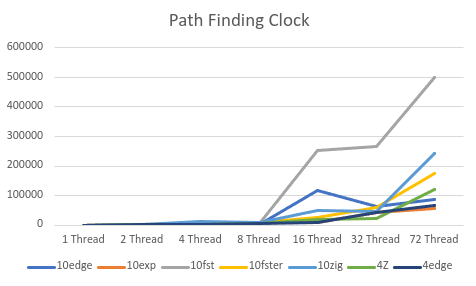
\includegraphics[width=\textwidth]{path-finding-clock.png}
\caption{Time Taken Overall Minus Time Taken Calculating Cell Cost}
\label{fig:5}
\end{figure}

\begin{table}[!htb]
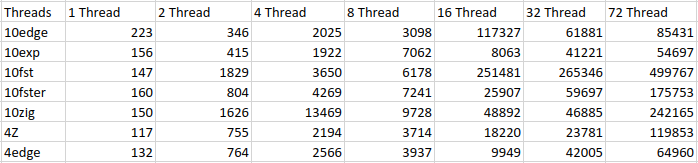
\includegraphics[width=\textwidth]{path-finding-clock-table.png}
\caption{Time Taken Overall Minus Time Taken Calculating Cell Cost}
\label{tab:5}
\end{table}

\begin{figure}[!htb]
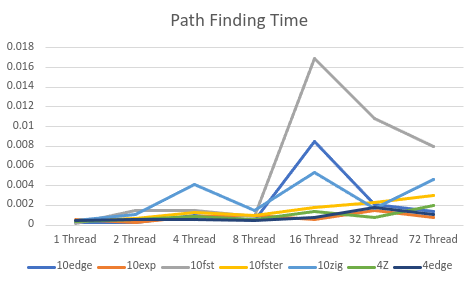
\includegraphics[width=\textwidth]{path-finding-time.png}
\caption{Clock Ticked Overall Minus Clock Ticked Calculating Cell Cost}
\label{fig:6}
\end{figure}

\begin{table}[!htb]
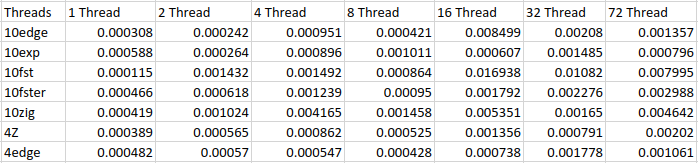
\includegraphics[width=\textwidth]{path-finding-time-table.png}
\caption{Clock Ticked Overall Minus Clock Ticked Calculating Cell Cost}
\label{tab:6}
\end{table}

\begin{table}[!htb]
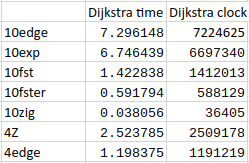
\includegraphics[width=10cm]{dijkstra-table.png}
\caption{Time and Clock tick taken by the sequential Dijkstra's algorithm}
\label{tab:7}
\end{table}

Figure \ref{fig:1} and Table \ref{tab:1} shows the amount of CPU time taken by each sample inputs
for each thread counts. CPU time excludes the time taken for IO and the time any core spent idling.

Figure \ref{fig:2} and Table \ref{tab:2} shows the amount of real world time that has elapsed since
the the algorithm started running til the algorithm has finished printing out all the results. This
includes the time taking to print the shortest path to stdout but does not include the time taken to
read the input in.

Figure \ref{fig:3} and Table \ref{tab:3} shows the amount of CPU time taken to calculate the cost of
all cells. This time also includes the time taken to calculate the delta. However, because
calculating the delta is just one single division and maximum reduce, the time of calculating the
cost should dominate the time measured and the extra time for calculating the delta should be
minimum.

Figure \ref{fig:4} and Table \ref{tab:4} shows the amount of real world time that has elapsed while
all cell costs are being calculated. This is measured at the same point as the CPU time for cell
cost.

Figure \ref{fig:5} and Table \ref{tab:5} shows the difference between the overall clock time taken
and the time taken to overall. The original intention of this data is to analyze the time taken by
the actual path finding algorithm. However, it appears to be dominated by noise.

Figure \ref{fig:6} and Table \ref{tab:6} shows the difference between the elapsed real world time
taken by the whole algorithm and the elapsed real world time taken by the cell costs evaluation.
These data again appears to be dominated by noise.

Table \ref{tab:7} shows both the elapsed real time taken and the amount of CPU time taken by the
sequential Dijkstra's algorithm. Those two measurements are somewhat duplicated because the
sequential algorithm only uses one core, so that core is busy most of the time and the CPU time ends
up being roughly proportional to each other.

\section*{Discussion}
Compared the overall time taken by my delta stepping algorithm \ref{tab:2} with a single thread, and
the overall time taken by the Dijkstra's algorithm \ref{tab:7}, we can see that for 10x10edge,
10x10expensive and 10x10fast, my delta stepping algorithm took roughly twice as long as the Dijkstra
algorithm. I believe this is due to the fact that the Dijkstra's algorithm only calculate the cell
costs needed to find the shortest path while my delta stepping algorithm always calculate all the
cell costs upfront. However, we can also see that for 10x10faster, 10x10zigzag, 4x4Z and 4x4edge, my
delta stepping algorithm performed significantly better than the Dijkstra's algorithm. I believe
this is due to the fact that the Dijkstra's algorithm calculate the cell costs from scratch
every time it needs to query it while my delta stepping algorithm only calculate each cell costs
once.

Nonetheless, when we look at my delta stepping algorithm with more than 2 threads \ref{tab:2}, we
can see that it ran significantly faster than the Dijkstra's algorithm. We can gain more insight
into the speed-up by looking into Table \ref{tab:6} and Figure \ref{fig:6}. Here we can see that the
vast majority of the time taken by the delta stepping algorithm are spent calculating the cell
costs. This make sense because cell costs are made to be intentionally expensive while the graph
itself is relatively small with only 100 nodes and less than 400 edges. As a result, the speed-up
we've obtained does not serve as a good source of analysis for generic parallel shortest path
algorithm because our result is dominated by an easily parallizable step. For future work, we can
test our algorithm without expensive cell cost calculation and with significantly larger graphs.

When we look at Figure \ref{fig:2} and Table \ref{tab:2}, we can see that in the case of 10x10edge
and 10x10expensive, the elapsed time roughly halves every time the number of thread doubles. This
make sense as those two input sample's calculation are heavily dominated by calculating the cell
costs. We can also see that for other input samples, the overall elapsed time in fact increases when
going from 32 threads to 72 threads and for some of them even from 16 threads to 32 threads. I
believe this is because for the node the algorithm running on are made up by 4 18 cores CPUs. As the
number of threads increase beyond 18, the algorithm can no longer run on a single CPU and therefore
the application starts incurring the communication costs between CPUs. If the algorithm doesn't
have a lot of easily parallizable task to do, it will spend most of its time on the communication
costs hence increasing the overall time taken by the algorithm.

When we look at Figure \ref{fig:1} and Table \ref{tab:1}, we can see that the total CPU time
increases as the number of threads increases. This is especially prevalent on small input sample
such as 4x4Z and 4x4edge where the CPU time more than doubled going from 32 thread to 72 threads.
This again matches with our earlier analysis of communication overhead between CPUs making the
algorithms slower instead of faster.

If we try to ignore the cell costs time and attempt to view the time taken to calculate the path
itself, we find very noisy data in Figure \ref{fig:6} and Table \ref{tab:6}. This is potentially due
to our flawed methodology of only doing one run per thread count per input sample instead of
averaging over multiple runs. If we try to ignore the noise in the data and attempt to view the
trend, we can see that the time of everything except cell costs calculation actually increases
significantly as the number of thread increases. I believe this is due to the fact that there isn't
a lot of work to be done with path finding, and, as mentioned above, that the communication overhead
between CPUs across sockets starts dominate the total running time. This communication overhead can
also explain the large amount of variation between each run. It could be that our algorithm are
sometimes being assigned to cores that are spread out among the sockets and sometimes assigned to
cores that are on the same sockets.

Speculating, if we increase the core count of the hardware the algorithm is running on as well and
the thread count of the algorithm to match the core count, the running time of the algorithm for
input 10x10expensive and 10x10edge would not see significant improvement after the core count exceed
100, as there are only 100 cell costs to calculate. If we increase the size of the graph well beyond
the core count and have cell costs calculation remain the dominating cost of the algorithm, we will
see a close to inversely proportional relationship between the running time and the core count with
some overhead as the core count increases due to communication overhead.

From a theoretical standpoint, if we discard the dominating factor that is the cell cost
calculation, my delta stepping algorithm should have a time complexity of $O((m+n)log^2(m*n))$ where
\(m\) and \(n\) are the width and height of the grid. This result is a specialization of the more
general result that is proven by Meyer and Sander in \cite{Meyer-1998} when the delta is chosen to
be \(\Theta(1/d)\) and the edge weights are uniformly distributed in \([0, 1]\). However, my
implementation of the algorithm did not take advantage many of the parallizable data structure
presented by Meyer and Sander \cite{Meyer-1998}. In particular, my buckets are implemented as C++
vectors which are not thread safe and have to be surrounded by locks to ensure their correctness.
When viewing the problem as a path finding problem rather than a cell cost calculating problem,
there are many improvements to be made to my algorithm.

\printbibliography

\end{document}
